\documentclass[a4paper,11pt,pdftex, parskip]{scrreprt}
\usepackage[pdftex]{graphicx}
\usepackage{ngerman}
\usepackage[utf8]{inputenc}
\usepackage[T1]{fontenc}
\usepackage{lmodern}
\usepackage[numbers]{natbib}
\usepackage[margin=5pt,font=small,labelfont=bf, textfont=it]{caption}
%\usepackage[reals]{layout}
\usepackage[lmargin = 2cm, rmargin = 2cm, tmargin = 2cm]{geometry}



\begin{document}
%\layout*
\begin{titlepage}

  
    \title{
        \begin{figure}[t]
            \centering
            
\includegraphics[scale = 0.125, keepaspectratio]{Logos/wwu_logo.png}
            
\includegraphics[scale = 0.5, keepaspectratio]{Logos/ifgi_logo.png}
        \end{figure}
        % \begin{figure}[t]
        %     \centering
        %     \begin{minipage}[b]{.4\linewidth}
        %         
\includegraphics[scale = 0.1, angle = 0]{Logos/wwu_logo.png}
        %        \end{minipage}
        %     \begin{minipage}[b]{.5\linewidth}
        %      
\includegraphics[scale = 0.4, angle = 0 ]{Logos/ifgi_logo.png}
        %     \end{minipage}
          
        %    \end{figure}
           
        \textnormal{ 
            \normalsize \Large 
            Westfälische Wilhelms Universität \\ Institut für Geoinformatik\\
            \vspace{3cm}
           % \LARGE 
            Proposal zu\\}
        \glqq {Semantische Kompression von Drohnenvideos \\ mit der Discrete Curve Evolution}\grqq 
        \vspace{1,5cm}}

   
    \author{ 
        Themensteller: Reinhard Moratz \\
        Betreuer: tbd. \\
        Ausgabetermin: tbd. \\
        \vspace{0.75cm}
        Abgabetermin: tbd. \\
        Vorgelegt von: Timo Lietmeyer \\
        Geboren am : 23.05.1999 \\
        E-Mail-Adresse: timolietmeyer@uni-muenster.de \\
        Matrikelnummer: 459 169 \\
        Studiengang: Bachelor Geoinformatik
    }
    \date{ }    
\end{titlepage}
\maketitle
%\tableofcontents

\section*{1 Motivation}
Drohnen mit Kameras verbreiten sich immer weiter in Deutschland. Durch die steigende Verbreitung von UAVs (Unmanned Aerial Vehicle) ist eine stabile Verbindung von Pilot zu Drohne von hoher Wichtigkeit \citep{Nehring2021}. \newline
Da bei der immer weiter voranschreitenden technischen Entwicklung abzusehen ist, dass die Kameraauflösung bei Drohnen weiter steigt \citep{futuretech2017}, ist auch eine stärkere Kompression dieser Bilder und Videos vonnöten, um eine stabile Verbindung weiter zu gewährleisten. Des Weiteren ist das Erreichen einer höheren Reichweite bei der Funkverbindung sehr wünschenswert. \newline
Im Rahmen dieser Bachelorarbeit soll beispielhaft eine Methode implementiert werden, die eine Kompression von Drohnenvideos ermöglicht.
% \begin{itemize}
%     \item Sequenzierung von Objekten kann für bessere (semantische) Kompression mithilfe der Discrete Curve Evaluation (DCE) benutzt werden 
%     \item bessere Reichweite, stabilere Funkverbindungen von Drohne zu Pilot 
%     \item Dadurch können auch private Drohnennutzer von besseren Bedingungen profitieren 
% \end{itemize}

\section*{2 Methodik}{
Zum Testen stellt der Betreuer Videomaterial, welches im Rahmen der Bachelorarbeit analysiert und komprimiert wird (s. Abb. \ref{Scr_ges_Vid}). Ein beispielhafter Verlauf ist in Abb. \ref{Bsp_Dorr} zu sehen. \\
Als ersten Schritt müssen die zu erkennenden Objekte detektiert werden (s. Abb. \ref{Scr_detail_Obj}). Bei dem Beispielvideo ist dies durch die statische Kameraposition in Verbindung mit den sich bewegenden Objekten durch Bewegtsegmentierung der beiden Objekte oder mit anderen Bilderkennungsalgorithmen, wie YOLO, möglich.\newline
Weitergehend müssen die detektierten Bildsegmente in eine Binärmaske umgewandelt werden, welche mit der DCE Methode vereinfacht werden kann. \newline
Das Umwandeln der segementierten Bildausschnitte in eine Binärmaske kann mithilfe eines Schwellwertverfahrens, welches von Nobuyuki Otsu entwickelt wurde, erfolgen \citep{Otsu1979}. Die weitere Vereinfachung des Polygons erfolgt dann mithilfe der Discrete Curve Evolution \citep{Barkowsky2000}
 

\begin{figure}[ht]
    \centering
    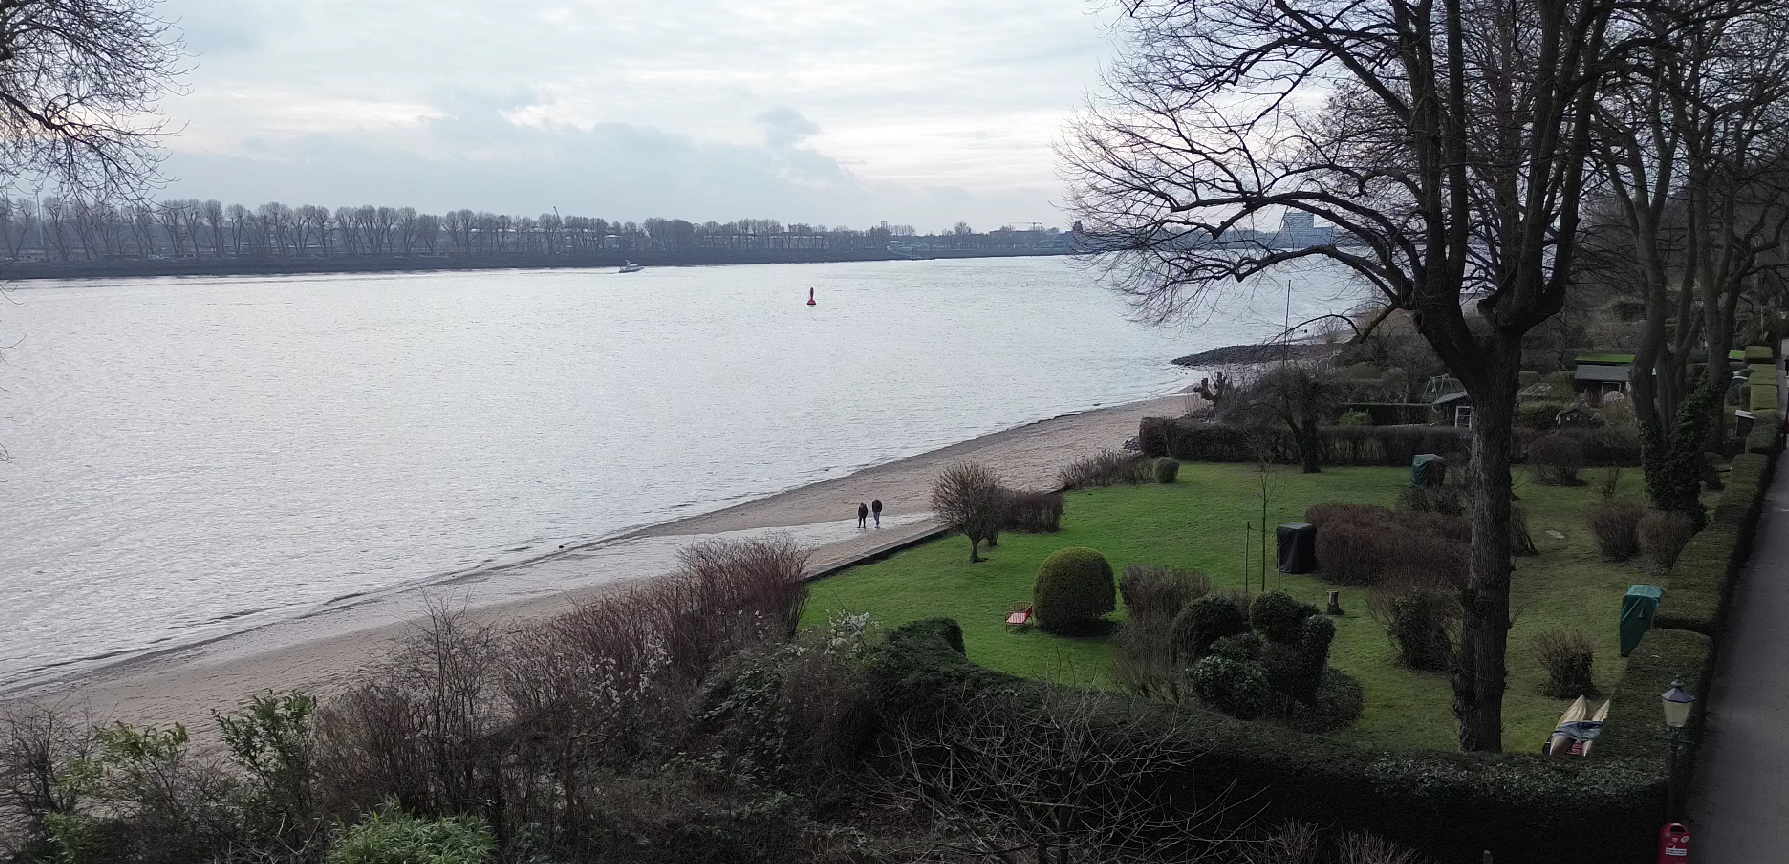
\includegraphics[scale=0.2, keepaspectratio]{images/screenshot_video_moratz.png}
    \caption[Screenshot des zu analysierenden Videos]{Screenshot des zu analysierenden Videos (Quelle: eigene Darstellung)}
    \label{Scr_ges_Vid}
\end{figure}
Die Discrete Curve Evolution berechnet anhand eines Grenzwertes, welche Punkte für die Darstellung einer Form irrelevant sind, sodass diese ohne größeren Informationsverlust entfernt werden können \citep{Barkowsky2000}. Durch die schrittweise Entfernung von Punkten kann eine bedarfsbezogene Vereinfachung des Polygons ermöglicht werden. \\
Anhand des komprimierten Videos, was als Ergebnis zu erwarten ist, kann eine Ergebnisevaluation stattfinden.
\begin{figure}[ht]
    \centering
    
\includegraphics[scale = 4, keepaspectratio] {images/detail_screenshot_people.png}
    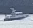
\includegraphics[scale = 4, keepaspectratio]{images/detail_screenshot_boat.png}
    \caption[Ausschnitte aus Abb. \ref{Scr_ges_Vid}, welche die beiden bewegenden Objekte darstellen ]{Ausschnitte aus Abb. \ref{Scr_ges_Vid}, welche die beiden bewegenden Objekte darstellen (Quelle: eigene Darstellung)}
    \label{Scr_detail_Obj}
\end{figure}
\begin{figure}[ht]
    \centering
    \includegraphics*[scale = 0.5, keepaspectratio]{images/Example_bird.png}
    \caption[Beispiel aus \citep{Dorr2017}]{Beispiel, welches einen segementierten Vogel zeigt, der in eine Binärmaske umgewandelt wird. Dieses Polygon wird dann mithilfe der DCE vereinfacht (Quelle: \citep{Dorr2017})}
    \label{Bsp_Dorr}
\end{figure}
}


% \begin{itemize}
    
%     \item Anwendung von DCE und semantischer Kompression mithilfe von Bilderkennungsalgorithmen (Yolo, etc.)
%     \item Binärmaske aus segementierten Bildmaterial mit Hilfe von  Schwellwertverfahren von Nobuyuki Otsu (möglw.)
    

% \end{itemize}



% \section*{3 Evaluation}
% \begin{itemize}
%     \item Hier kommt ein Evaluationsstichpunkt
%     \item Anwendung auf von Betreuer zur Verfügung gestelltes Videomaterial
% \end{itemize}


\section*{3 Ausblick}
Wenn das Ergebnis der Komprimierung von Drohnenvideos mithilfe der Discrete Curve Evolution zufriedenstellend ist, kann eine hardwarenähere Programmierung erfolgen. Diese könnte in C oder C++ gemacht werden, um schnellere Ergebnisse liefern zu können, da die Prozessierungsgeschwindigkeit von Python begrenzt ist.\newline
Durch die hardwarenähere Implementierung der DCE könnte eine Komprimierung direkt am Aufzeichnungsort, bzw. in der Drohne, stattfinden, welche die Datenübertragungsrate senkt. Durch die Senkung der Datenübertragungsrate kann eine stabilere Funkverbindung, sowie höhere Reichweite ermöglicht werden.


% \begin{itemize}
%     \item Hier kommt ein Ausblickstichpunkt
%     \item Machbarkeitsstudie der DCE und semantischer Kompression auf Verbesserung der Verbindung zwischen Pilot und Drohne
%     \item Anwendung in C/C++, bzw. hardwarenaher umschreiben, damit schnellere (VorOrt-) Prozessierung/Kompression möglich ist
%     \item praktisches Beispiel entwicklen / eigene Drohnensoftware implementieren
% \end{itemize}

\appendix


\bibliographystyle{plainnat}
\bibliography{Bibliography}
\pagenumbering{roman}
\setcounter{page}{1}
\listoffigures



\end{document}